\documentclass{exam}
\usepackage[utf8]{inputenc}
\usepackage{lmodern}
\usepackage{microtype}

% \usepackage[parfill]{parskip}
\usepackage[dvipsnames]{xcolor}
\usepackage{amsmath}
\usepackage{amsfonts}
\usepackage{amsthm}
\usepackage{siunitx}
\DeclareSIUnit\year{yr}
\DeclareSIUnit\foot{ft}
\DeclareSIUnit\litre{\liter}

\usepackage{skull}

\usepackage{pgfplots}
\usepgfplotslibrary{polar}
\pgfplotsset{compat=1.11}
\usepgfplotslibrary{statistics}
\usepackage{graphicx}
\usepackage{sidecap}
\sidecaptionvpos{figure}{c}
\usepackage{float}
\usepackage{gensymb}
\usepackage{tkz-euclide}
\usetkzobj{all}
\usepackage{commath}
\usepackage{hyperref}
\usepackage{enumitem}
\usepackage{wasysym}
\usepackage{multicol}
\usepackage{mathtools}
\usepackage{tcolorbox}
\usepackage{tabularx}
\usepackage[version=4]{mhchem}
\usepackage{changepage}
\usepackage{listings}
\lstset{basicstyle=\ttfamily\linespread{0.8}\small}

\renewcommand*{\thefootnote}{\fnsymbol{footnote}}

\newtheorem*{thm}{Theorem}
\newtheorem*{iden}{Identity}
\newtheorem*{lemma}{Lemma}
\newtheorem{obs}{Observation}
\theoremstyle{definition}
\newtheorem*{defn}{Definition}
\newtheorem*{ex}{Example}
\newtheorem{con}{Construction}
\newtheorem*{alg}{Algorithm}

\newtheoremstyle{break}
  {\topsep}{\topsep}%
  {\itshape}{}%
  {\bfseries}{}%
  {\newline}{}%
\theoremstyle{break}
\newtheorem*{bthm}{Theorem}

% russian integral
\usepackage{scalerel}
\DeclareMathOperator*{\rint}{\scalerel*{\rotatebox{17}{$\!\int\!$}}{\int}}

% \DeclareMathOperator*{\rint}{\int}

\pgfplotsset{vasymptote/.style={
    before end axis/.append code={
        \draw[densely dashed] ({rel axis cs:0,0} -| {axis cs:#1,0})
        -- ({rel axis cs:0,1} -| {axis cs:#1,0});
    }
}}

% \pointsinrightmargin
\boxedpoints
\pointname{}

\newcommand{\questioA}{\question[\texttt{\textbf{\color{Cerulean} A}}]}
\newcommand{\questioM}{\question[\texttt{\textbf{\color{PineGreen} M}}]}
\newcommand{\questioE}{\question[\texttt{\textbf{\color{WildStrawberry} E}}]}
\newcommand{\questioS}{\question[\texttt{\textbf{\color{Goldenrod} S}}]}
\newcommand{\questioO}{\question[\texttt{\textbf{\color{BurntOrange} O}}]}

\newcommand{\parA}{\part[\texttt{\textbf{\color{Cerulean} A}}]}
\newcommand{\parM}{\part[\texttt{\textbf{\color{PineGreen} M}}]}
\newcommand{\parE}{\part[\texttt{\textbf{\color{WildStrawberry} E}}]}
\newcommand{\parS}{\part[\texttt{\textbf{\color{Goldenrod} S}}]}
\newcommand{\parO}{\part[\texttt{\textbf{\color{BurntOrange} O}}]}

\newcommand{\subparA}{\subpart[\texttt{\textbf{\color{Cerulean} A}}]}
\newcommand{\subparM}{\subpart[\texttt{\textbf{\color{PineGreen} M}}]}
\newcommand{\subparE}{\subpart[\texttt{\textbf{\color{WildStrawberry} E}}]}
\newcommand{\subparS}{\subpart[\texttt{\textbf{\color{Goldenrod} S}}]}
\newcommand{\subparO}{\subpart[\texttt{\textbf{\color{BurntOrange} O}}]}

\newcommand{\mainHeader}[2]{\section*{NCEA Level 2 Mathematics\\#1. #2}}
\newcommand{\mainHeaderHw}[2]{\section*{NCEA Level 2 Mathematics (Homework)\\#1. #2}}
\newcommand{\seealso}[1]{\begin{center}\emph{See also #1.}\end{center}}
\newcommand{\drills}[1]{\begin{center}\emph{Drill problems: #1.}\end{center}}
\newcommand{\basedon}[1]{\begin{center}\emph{Notes largely based on #1.}\end{center}}


\begin{document}

\mainHeader{1}{Coordinate Geometry}
The ancient Greeks were doing geometry at least as early as the 7th century BCE: Euclid's \textit{Elements}, a mathematical book containing a collection
of geometric propositions and proofs, is arguably the most influential mathematical work of all time and was regularly taught in schools until the 19th
century. Of course, there have been some revolutions in geometry since the time of Euclid, and one of the most important was an idea due to Ren\'e Descartes
(``Renay Daycart'') who first published the idea of using a coordinate system in 1637, in his book \textit{La G\'eom\'etrie}.

The idea is relatively simple: assign every point in the plane two numbers (coordinates) that describe its location with respect to the coordinate axes.

\begin{center}
  \fbox{\begin{tikzpicture}
    \begin{axis}[
      axis lines = center,
      xlabel = $ x $,
      ylabel = $ y $,
      xmin = -5, xmax = 5,
      ymin = -5, ymax = 5
    ]
      \node[label={180:{(2,3)}},circle,fill,inner sep=2pt] at (axis cs:2,3) {};
    \end{axis}
  \end{tikzpicture}}
\end{center}

Traditionally, the two axes are the $ x$- and $ y$- axes; in three dimensions, we add a $ z$-axis as well, at right angles to the first two.

The reason this idea is so powerful is that now we can represent geometric objects algebraically, by writing down an equation so that the coordinates
of every point of our object satisfies the equation.

For example, the equations $ y = 3x + 2 $ (red) and $ y = \frac{1}{2x} $ (blue) are graphed here.
\begin{center}
  \fbox{\begin{tikzpicture}
    \begin{axis}[
      axis lines = center,
      xlabel = $ x $,
      ylabel = $ y $
    ]
      \addplot[domain = -5:5, color = red] {3*x + 2};
      \addplot[domain = -5:-0.05, color = blue, style=dashed] {1/(2*x)};
      \addplot[domain = 0.05:5, color = blue, style=dashed] {1/(2*x)};
    \end{axis}
  \end{tikzpicture}}
\end{center}

\subsection*{Points}
One thing that we can do within a coordinate system is define the concept of ``distance'' between two points. We will do this by taking our two
points and drawing a right-angled triangle, as follows:

\begin{center}
  \fbox{\begin{tikzpicture}
    \begin{axis}[
      axis lines = center,
      xlabel = $ x $,
      ylabel = $ y $,
      xmin = -5, xmax = 5,
      ymin = -5, ymax = 5
    ]
      \node[label={180:{$A(2,3)$}},circle,fill,inner sep=2pt] at (axis cs:2,3) {};
      \node[label={180:{$B(-1,-2)$}},circle,fill,inner sep=2pt] at (axis cs:-1,-2) {};
      \draw[] (2,3) -- (-1,-2) -- (2,-2) -- (2,3);
    \end{axis}
  \end{tikzpicture}}
\end{center}

Then the distance between the two points $ A $ and $ B $ is given by Pythagoras' theorem:-
\begin{displaymath}
  d(A,B) = \sqrt{(3 - -2)^2 + (2 - -1)^2}.
\end{displaymath}

More generally, the distance between two points $ A(x_0, y_0) $ and $ B(x_1, y_1) $ is given by
\begin{displaymath}
  d(A,B) = \sqrt{(x_0 - x_1)^2 + (y_0 - y_1)^2}.
\end{displaymath}

We can also find the midpoint of two points: the point precisely halfway between them. Clearly, if a point is halfway
between two points on the plane then it is halfway between the two points on both coordinate axes; hence the point
halfway between two points $ A(x_0, y_0) $ and $ B(x_1, y_1) $ is given by
\begin{displaymath}
  m(A,B) = \left(\frac{x_0 + x_1}{2}, \frac{y_0 + y_1}{2}\right).
\end{displaymath}

\clearpage
\subsection*{Lines}
Turning to lines now, it is fairly obvious that every line (when we mention lines, we of course always mean \emph{straight lines}) has
a `slope'. The slope (or `gradient') of a line is a number which describes how `steep' the line is. We define the `slope' of a line to be the `distance
a point on the line travels upwards, as we move to the right by one unit length'. For example, consider the line in red here.
\begin{center}
  \fbox{\begin{tikzpicture}
    \begin{axis}[
      axis lines = center,
      xlabel = $ x $,
      ylabel = $ y $,
      xmin = -5, xmax = 5,
      ymin = -5, ymax = 5
    ]
      \node[label={180:{$A(2,3)$}},circle,fill,inner sep=2pt] at (axis cs:2,3) {};
      \node[label={180:{$B(-1,-2)$}},circle,fill,inner sep=2pt] at (axis cs:-1,-2) {};
      \addplot[domain = -5:5, color = red] {(5/3)*(x - 2) + 3};
      \draw[] (-1,-2) -- (2,-2) -- (2,3);
    \end{axis}
  \end{tikzpicture}}
\end{center}
The slope of this line is $ \frac{3 - -2}{2 - -1} = \frac{5}{3} $: every three steps to the right, we move five steps up --- so if we move
one step to the right, we move $ 5/3 $ of a step up.

We can use this idea to write down the equation of a line in general. Note that we have to take for granted one thing:
\begin{center}
  \emph{There is precisely one line through any two points.}
\end{center}
We can't \emph{prove} this within our conception of what it means to be a geometry, it is an axiom (something we assume without proof to be true).
Note, however, that it is possible to define geometry in general in a different way so that this does become a theorem (something with a proof), but
this requires other axioms beneath it that we cannot prove.

From our discussion above, we know that the slope of the line through the points $ (x_0, y_0) $ and $ (x_1, y_1) $ is given by
\begin{displaymath}
  \frac{y_1 - y_0}{x_1 - x_0} \left(= \frac{\text{rise}}{\text{run}}\right).
\end{displaymath}

We can now prove the following:

\begin{thm}
  The unique line through the points $ (x_0, y_0) $ and $ (x_1, y_1) $ is given by the linear equation
  \begin{displaymath}
    y - y_0 = \frac{y_1 - y_0}{x_0 - x_1} (x - x_0) = m(x - x_0),
  \end{displaymath}
  where $ m $ is the slope of the line.
\end{thm}
\begin{proof}
  Let $ (x,y) $ be any point on the line. We need to find an expression for $ y $ in terms of $ x $. However, note that the slope of the
  line between $ (x,y) $ and $ (x_0,y_0) $ is the same as the slope between $ (x_0,y_0) $ and $ (x_1, y_1) $ (because the line is straight).
  Therefore, we have
  \begin{displaymath}
    \frac{y - y_0}{x - x_0} = \frac{y_1 - y_0}{x_0 - x_1}
  \end{displaymath}
  and rearranging this, we have
  \begin{displaymath}
    y - y_0 = \frac{y_1 - y_0}{x_0 - x_1}(x - x_0),
  \end{displaymath}
  Q.E.D.
\end{proof}

For example, the line through $ (2,1) $ and $ (3,4) $ has slope $ \frac{4 - 1}{3 - 2} = 3 $, and equation
\begin{displaymath}
  y - 1 = 3(x - 2).
\end{displaymath}
On the other hand, we could swap around the two points and write the equation
\begin{displaymath}
  y - 4 = 3(x - 3).
\end{displaymath}

This is slightly annoying: both describe the same line, so why do we have two equations? Well, we can rearrange them:
\begin{gather*}
  y - 1 = 3(x - 2) \implies y = 3(x - 2) + 1 \implies y = 3x - 6 + 1 \implies y = 3x - 5;\\
  y - 4 = 3(x - 3) \implies y = 3(x - 3) + 4 \implies y = 3x - 9 + 4 \implies y = 3x - 5.
\end{gather*}
So the equations are the same if we carry out this process of putting them into the form
\begin{displaymath}
  y = mx + c
\end{displaymath}
where $ m $ is still the slope of the line, and $ c $ is the $ y$-coordinate of the place where the line crosses the $ y$-axis (since
this point is the point on the line where $ x = 0 $ and so $ y = m0 + c = c $).

\subsection*{Questions}
\begin{questions}
  \question Find the distance between the following pairs of points, drawing a diagram for each showing the geometric meaning of the
            thing you are calculating.
    \begin{parts}
      \part $(3,4)$ and $(6,8)$
      \part $(3,0)$ and $(0,4)$
      \part $(-1,1)$ and $(-4,-4)$
      \part $(-4,-4)$ and $(-1,1)$
    \end{parts}
  \question Justify the following statements mathematically, where $ A $ and $ B $ are points.
    \begin{parts}
      \part The distance from $ A $ to $ B $ is the same as the distance from $ B $ to $ A $.
      \part The distance from the midpoint of $ A $ and $ B $ ($m(A,B)$) to $ A $ is the same as the distance from $ m(A,B) $ to $ B $.
      \part The equation of the line describing the $ y$-axis is $ x = 0 $, and the equation of the line describing the $ x$-axis is $ y = 0 $.
      \part The slope of a horizontal line is zero.
      \part A vertical line does not have a well-defined slope.
      \part A line with a negative slope is sloping downwards.
    \end{parts}
  \question Find the slope of the line through the following points.
    \begin{parts}
      \part $(5,7)$ and $(-2,1)$
      \part $(-2,1)$ and $(5,7)$
      \part $\left(\frac{2}{3},1\right)$ and $(4,2)$
      \part $(2\pi,1)$ and $(0,\pi + 1)$
    \end{parts}
  \question Find the points where the line $ y = -3x + 2 $ crosses the $ x$- and $ y-$axes. These are called the $ x$- and $ y$-intercepts.
  \question Find the point where the line $ y = -x + 2 $ crosses the line $ y = x + 2 $.
  \question Justify intuitively the ``triangle inequality'', if $ A $, $ B $, and $ C $ are any three points:
            \begin{equation}
              d(A,B) \leq d(A,C) + d(C,B). \tag{Triangle inequality}
            \end{equation}
  \question Two lines are \emph{perpendicular} if the angle between them is a right angle. Show that if the gradient of a line is $ m $
            then the gradient of any perpendicular line is $ -1/m $.
  \question Two lines are \emph{parallel} if they do not intersect. Show that two lines are parallel if and only if they have the same gradient.
  \question Let $ AB $ be some line segment. The perpendicular bisector of $ AB $ is the (unique) line perpendicular to $ AB $ and passing
            through $ m(A,B) $.
    \begin{parts}
      \part Find the equation of the perpendicular bisector of the segment joining $ (3,2) $ and $ (2,5) $.
      \part In general, if $ A = (A_x, A_y) $ and $ B = (B_x, B_y) $, find the equation of the perpendicular bisector of $ AB $.
    \end{parts}
  \question Let $ ABCD $ be a quadrilateral, such that $ d(A,B) = d(B,C) $ and $ d(C,D) = d(D,A) $. Show that the line $ AC $ is
            the perpendicular bisector of the segment $ BC $.
  \question In three dimensions, we can define the distance between two points $ (x_0,y_0,z_0) $ and $ (x_1,y_1,z_1) $ using the 3D version
            of Pythagoras' theorem:
            \begin{displaymath}
              d(A,B) = \sqrt{(x_0 - x_1)^2 + (y_0 - y_1)^2 + (z_0 - z_1)^2}.
            \end{displaymath}
            (We will prove this version of Pythagoras' theorem in three dimensions in a few weeks.)
    \begin{parts}
      \part Show that the distance between two points on the $ x,y$-plane (the plane $ z = 0 $) reduces to the 2D version we gave above.
      \part Write down a plausible definition for the midpoint of $ A $ and $ B $ in three dimensions.
      \part Using your definition, find the midpoint of $ A(2,-2,5) $ and $ B(6,8,9) $; is the distance between the midpoint and $ A $
            half the distance between $ A $ and $ B $?
    \end{parts}
  \question Which of the following triangles $ ABC $ are isosceles or right-angled (or both)?
    \begin{parts}
      \part $ A = (1,3) \quad B = (4,-2) \quad C = (1,-2) $
      \part $ A = (1,-5) \quad B = (2,-1) \quad C = (9,-6) $
      \part $ A = (4,0) \quad B = (8,2) \quad C = (8,-2) $
    \end{parts}
  \question Consider the three points $ (2,4) $, $ (-1,8) $, and $ (6,-3) $. Compute the equations
            for the perpendicular bisectors of each side, and show that all three bisectors intersect
            at a single point. Does this happen for every triangle?
  \question Let $ ABCD $ be a quadrilateral. Show that the quadrilateral $ WXYZ $, where
            \begin{gather*}
              W = m(A,B)\\
              X = m(B,C)\\
              Y = m(C,D)\\
              Z = m(D,A),
            \end{gather*}
            is a parallelogram.
  \clearpage
  \question Challenge problem 1. Let $ ABCD $ be a parallelogram. Draw a square on each side of the parallelogram, and choose
            the centre of each of the squares. Show that these centres form the vertices of a larger square. Show that the diagonals
            of this square intersect at the same point as the diagonals of $ ABCD $.
  \question Challenge problem 2. Consider a tetrahedron (see the figure below and \texttt{tetrahedron.ggb}). For each pair of opposite sides, draw
            a line segment connecting their midpoints.
            \begin{center}
              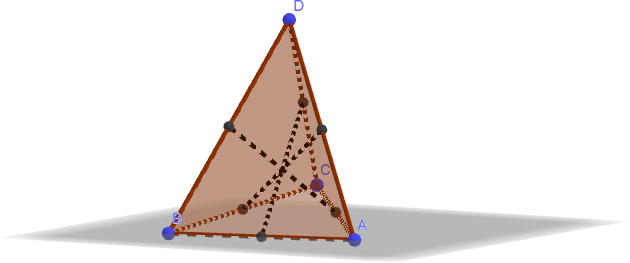
\includegraphics[width=0.4\textwidth]{tetrahedron}
            \end{center}
    \begin{parts}
      \part Show that all three such line segments intersect at a single point.
      \part In what ratio does the point of intersection divide each segment?
    \end{parts}
\end{questions}

\end{document}
